\documentclass[aspectratio=169]{beamer}
\usepackage[utf8]{inputenc}
\usepackage{graphicx}
\usepackage{color}
\usepackage{graphicx}
\usepackage{fancybox}
\usepackage[ruled,vlined]{algorithm2e}
\usepackage{standalone}
\usepackage{tikz}
\usetikzlibrary{shapes,arrows.meta}
%\usepackage{enumitem}

\usepackage{beamerthemesplit}
\usetheme[compress]{Heidelberg}
\definecolor{unirot}{rgb}{0.5976525,0,0}
\usecolortheme[named=unirot]{structure}

\title{GPGPU Accelerated Iterative Filtering of Scalar Fields on Discrete Manifolds}
\author{Bryan Wolfford}

\institute[Uni HD]{
	Universität Heidelberg\\
	Interdisciplinary Center for Scientific Computing\\
	Forensic Computational Geometry Laboratory\\
	\color{unirot}{wolfford@stud.uni-heidelberg.de}
}
\date{\today}

\AtBeginSection[]{
	\begin{frame}<beamer> 
		\frametitle{Outline}
		% show TOC and highlight current section
		\tableofcontents[currentsection]  
	\end{frame}
}

%\AtBeginSubsection[]{
%	\begin{frame}<beamer> 
%		\frametitle{Outline}
		% show TOC and highlight current section
%		\tableofcontents[currentsection,currentsubsection]  
%	\end{frame}
%}

\begin{document}
\newcommand{\fors}[1]{#1he Fast One-Ring smoothing filter}
\newcommand{\Fors}[1]{#1he Fast One-Ring smoothing filter for scalar fields on discrete manifolds}
\newcommand{\tdd}{3D-data}
\newcommand{\wmfv}[1]{weighted mean function value#1}
%
\newcommand{\bE}{\mathcal{E}}
\newcommand{\bF}{\mathcal{F}}
\newcommand{\bM}{\mathcal{M}}
\newcommand{\bN}{\mathcal{N}}
\newcommand{\bO}{\Omega}
\newcommand{\bP}{\mathcal{P}}
\newcommand{\bR}[1]{\mathbb{R}^{#1}}
\newcommand{\bT}{\mathcal{T}}
\newcommand{\bc}{\mathbf{c}}
\newcommand{\bp}{\mathbf{p}}
\newcommand{\bs}{\mathbf{s}}
\newcommand{\bt}{\mathbf{t}}
\newcommand{\bv}{\mathbf{v}}
%
\newcommand{\elm}{\ell_\text{min}}
\newcommand{\gelm}{\overline{\elm}}
\newcommand{\ellstar}{\ell_\ast}
%
\newcommand{\fM}{\mathfrak{M}}
%
\newcommand{\mbeq}{\overset{!}{=}}
%
\newcommand{\sipo}{i\kern-.7pt\scalebox{0.66}{+}\kern-1.2pt1}
\newcommand{\sipt}{i\kern-.7pt\scalebox{0.66}{+}\kern-1.2pt2}
\newcommand{\sjpo}{j\kern-.7pt\scalebox{0.66}{+}\kern-1.2pt1}
\newcommand{\sjpt}{j\kern-.7pt\scalebox{0.66}{+}\kern-1.2pt2}
\newcommand{\sps}{\kern-2pt+\kern-3pt}
\newcommand{\sxpx}[2]{#1\kern-.7pt\scalebox{0.66}{+}\kern-1.2pt#2}
\newcommand{\sv}[1]{v,\kern.75pt #1}
%
\newcommand{\todoRemove}[1]{\todo[color=red!40]{Remove: #1}}
\newcommand{\todoAsk}[1]{\todo[color=yellow!40]{Ask: #1}}
\newcommand{\todoCitation}[1]{\todo[color=teal!40]{Cite: #1}}
\newcommand{\todoReference}[1]{\todo[color=lime!40]{Ref: #1}}
\newcommand{\todoResearch}[1]{\todo[color=magenta!40]{Research: #1}}
\newcommand{\todoBackground}[1]{\todo[color=violet!40]{Bg: #1}}
\newcommand{\todoReword}[1]{\todo[color=cyan!40]{Reword: #1}}
\newcommand{\todoStyle}[1]{\todo[color=pink!40]{Style: #1}}
%xcolor base colors:
%	black
%	blue
%	brown
%%%	cyan
%%%	lime
%%%	magenta
%	olive
%	orange
%%%	pink
%	purple
%%%	red
%%%	teal
%%%	violet
%	white
%%%	yellow

\definecolor{MyTeal}{rgb}	{0, 	.5, 	.5}		%teal = 0,127,127
\definecolor{MyLtTeal}{rgb}	{.8125, .9375, 	.9375}	%lt.teal = 207,239,239
\definecolor{MySand}{rgb}	{1, 	.625, 	0}		%sand = 255,159,0
\definecolor{MyLtSand}{rgb}	{1, 	.9766, 	.875}	%lt.sand = 255,249,223
\definecolor{MyCoral}{rgb}	{1, 	.375, 	.375}	%coral = 255,96,96
\definecolor{MyLtCoral}{rgb}{1, 	.875, 	.875}	%lt.coral = 255,223,223

\frame[plain]{\titlepage}
\frame{\frametitle{Outline}\tableofcontents}




%================================================
%================================================
\section{Introduction \& Motivation}

%------------------------------------------------
\frame{
\frametitle{Introduction}

}

%------------------------------------------------
\frame{
\frametitle{One-Ring Neighborhoods in Regular and Irregular Meshes}
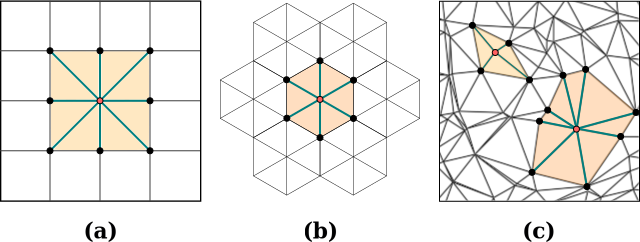
\includegraphics[width=1.0\linewidth]{../figures/neighborhoods.png}
}

%------------------------------------------------
\frame{
\frametitle{SIMD Architecture}
\includegraphics[width=1.0\linewidth]{../figures/tikz/simdArchitecture.pdf}
}

%------------------------------------------------
\frame{
\frametitle{CPU vs GPU Construction}
\includegraphics[width=1.0\linewidth]{../figures/cpuvgpu.png}
}




%================================================
%================================================
\section[FORS]{Fast One-Ring Smoothing}


%================================================
\subsection[Foundation]{Mathematical Foundation}

%------------------------------------------------
\frame{
\frametitle{A One-Ring Neighborhood and its Geodesic Disc}
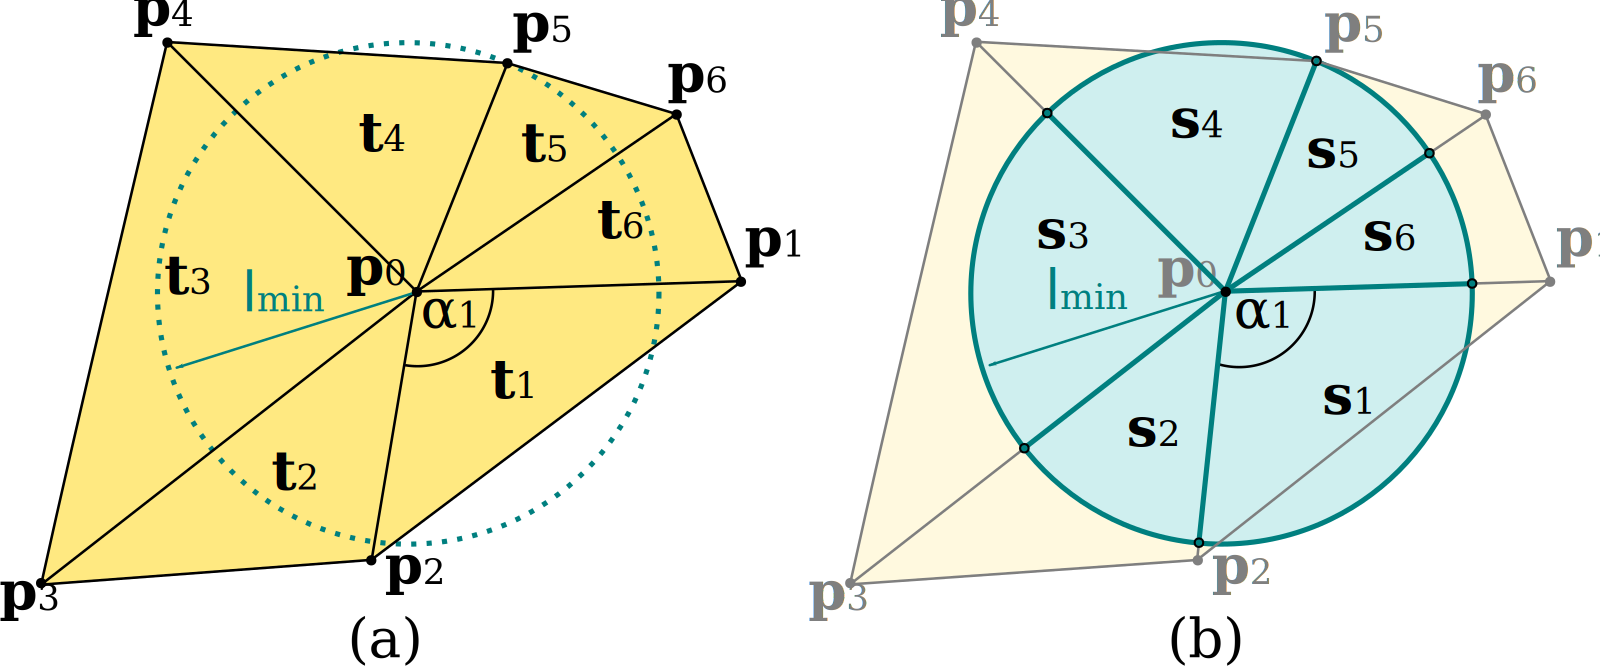
\includegraphics[width=1.0\linewidth]{../figures/geodesicDisc.png}
}

%------------------------------------------------
\frame{
\frametitle{An Enhanced View of a Circle Sector}
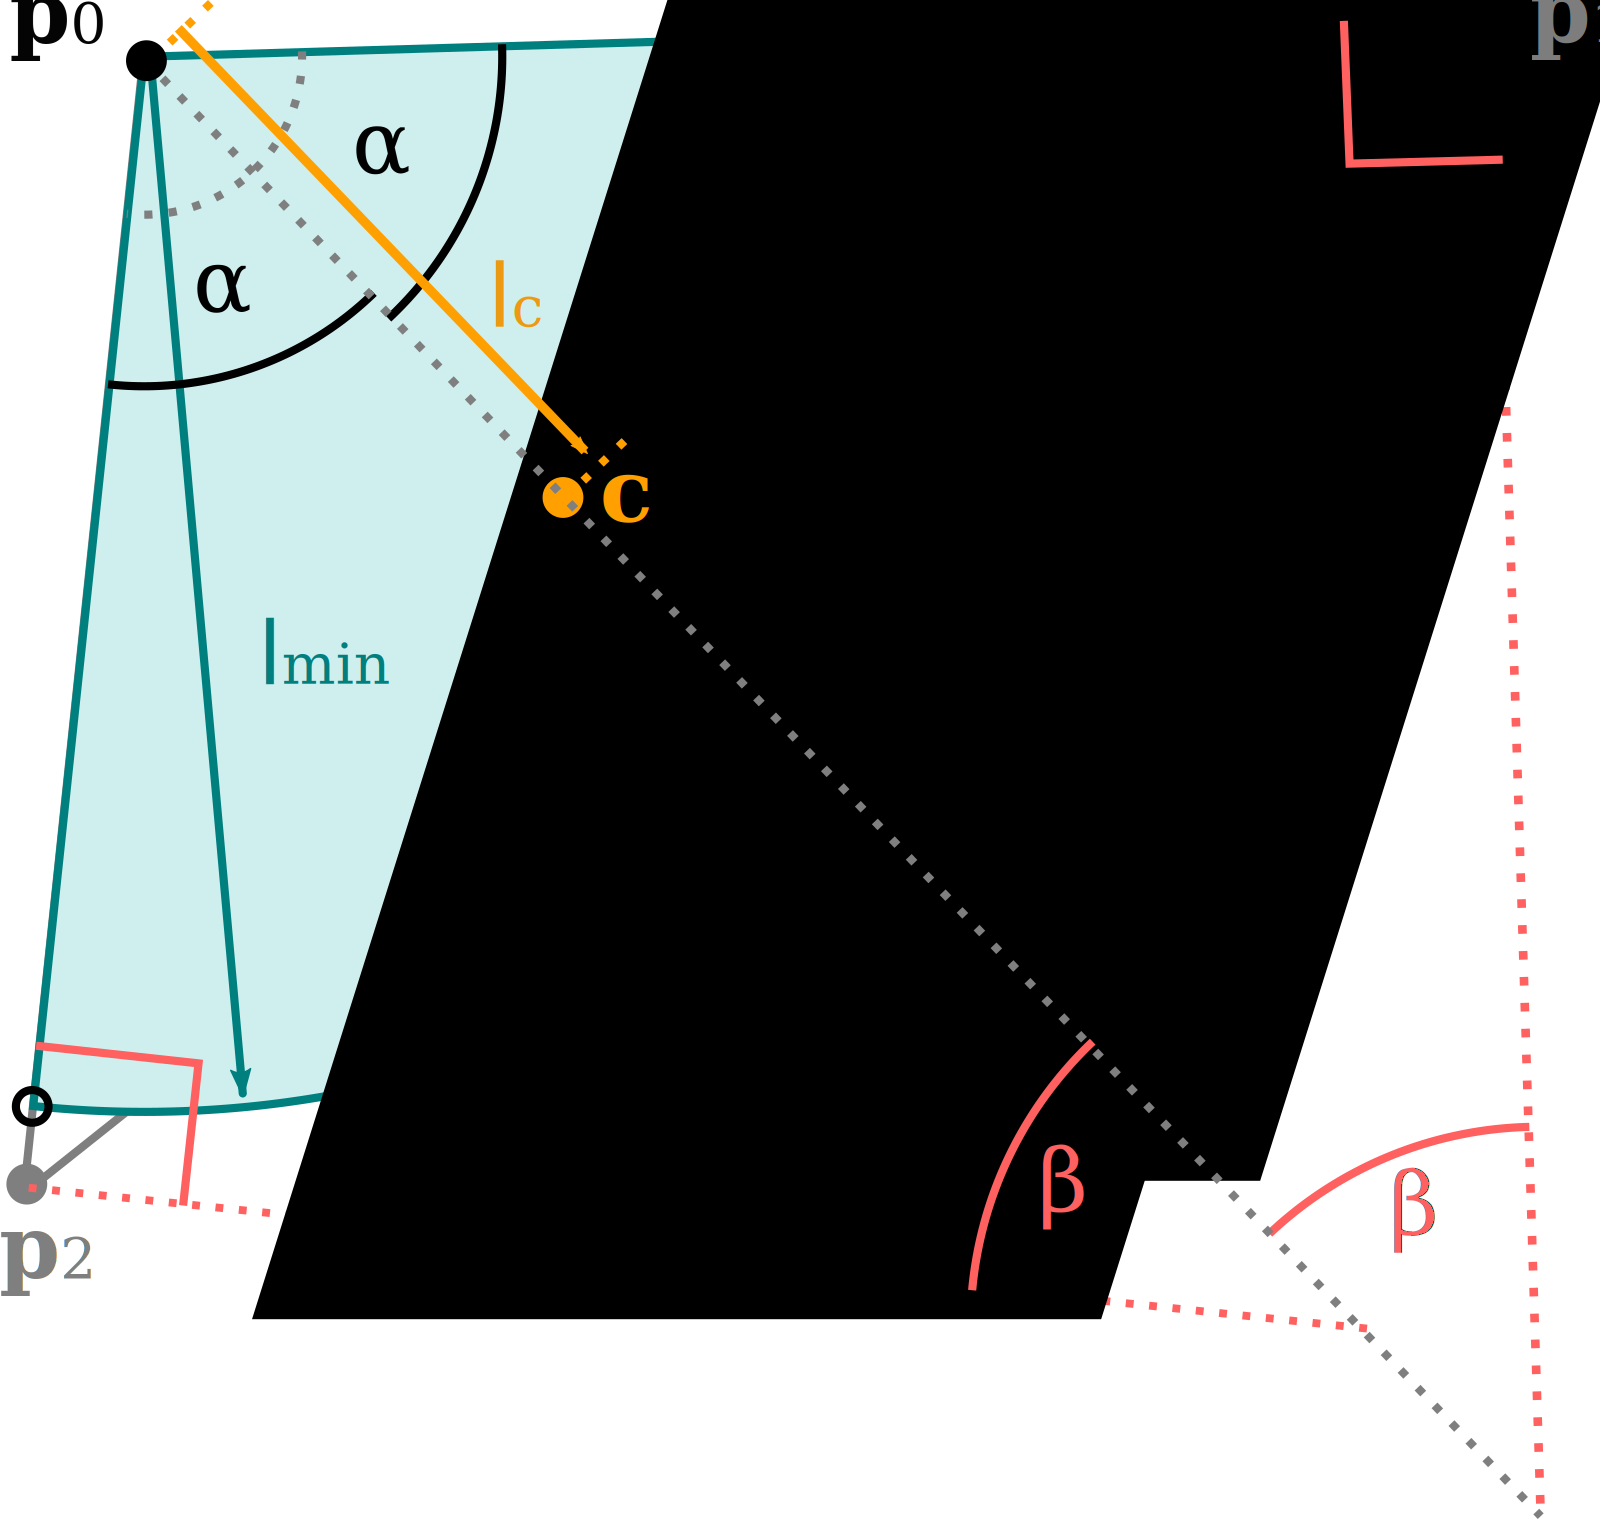
\includegraphics[width=0.5\linewidth]{../figures/anglesAndCenterOfGravity.png}
}

%------------------------------------------------
\frame{
\frametitle{Interpolation of Function Values toward the Center of Gravity}
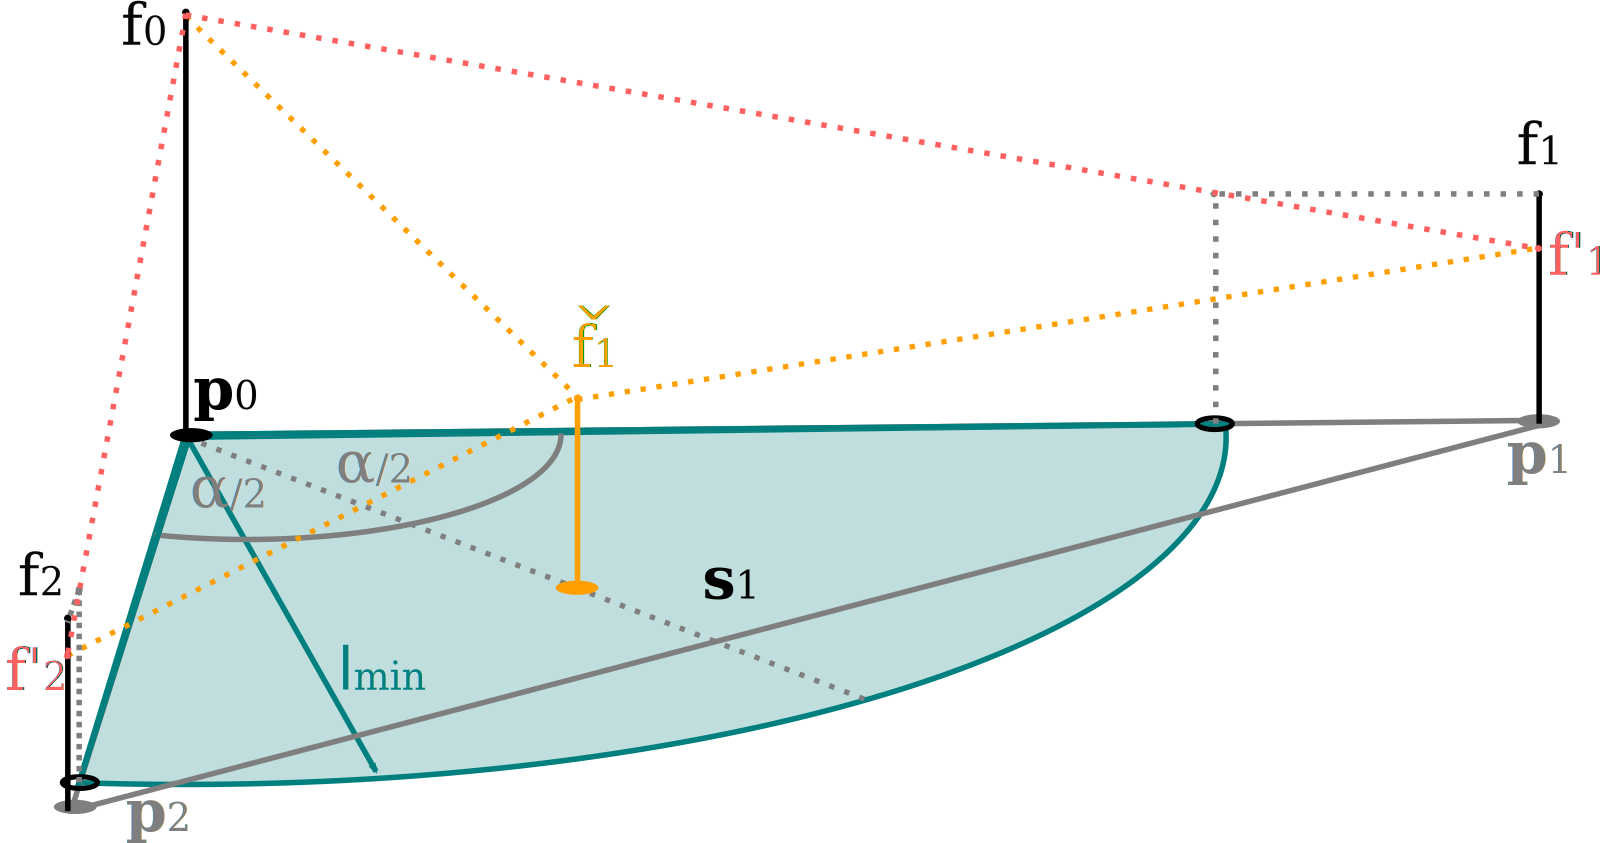
\includegraphics[width=1.0\linewidth]{../figures/interpolatedFunctionValues.png}
}

%------------------------------------------------
\frame{
\frametitle{Weighted Mean Function Value $f'_v$at $\bp_v$}
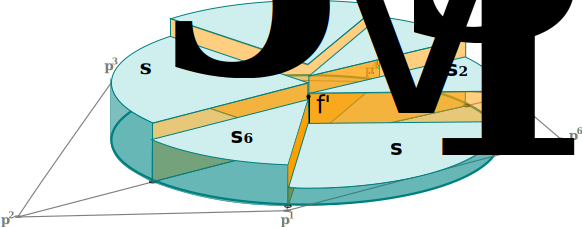
\includegraphics[width=1.0\linewidth]{../figures/funcValVolumes.png}
}


%================================================
\subsection[Serial]{Serial Algorithm}

%------------------------------------------------
\frame{
\frametitle{Union Operations as Performed in Build Neighborhoods}
\includestandalone[width=\textwidth]{../figures/tikz/unionsOfSimpleBuildNeighborhoods}
}


%================================================
\subsection[Parallel]{Parallel Algorithm}

%------------------------------------------------
\frame{
\frametitle{Parallel Algorithm}

}




%================================================
%================================================
\section{Experiments \& Evaluation}


%================================================
\subsection{Filter Response}

%------------------------------------------------
\frame{
\frametitle{Experiment 1}

}


%================================================
\subsection{Parallel Algorithm}

%------------------------------------------------
\frame{
\frametitle{Experiment 1}

}




%================================================
%================================================
\section[Conclusion]{Conclusion \& Outlook}

%------------------------------------------------
\frame{
\frametitle{Conclusion}

}

%------------------------------------------------
\frame{
\frametitle{Outlook}

}

%------------------------------------------------
\frame{
\frametitle{Questions}

\begin{figure}
	
\includegraphics[width=.8\textwidth]{questions} 
\end{figure}
\vspace*{-3.3cm}\begin{center}\begin{LARGE}\textbf{Questions}\end{LARGE}\end{center}
\vspace*{2cm}
}

\end{document}
